
\chapter{Gardez les pieds sur Terre}
Plut\^ot que de placer notre terrain comme une simple entit\'e dans la sc\`ene (ce qui serait tr\`es laborieux), Ogre propose de passer par une classe Terrain pour la gestion des terrains dans la sc\`ene.

Le terrain n'est g\'en\'eralement pas seul et le ciel joue un r\^ole important pour le r\'ealisme de la sc\`ene. L\`a encore, quelques outils bienvenus offrent diff\'erentes solutions pour obtenir un r\'esultat convaincant.



\section{Cr\'eer un terrain}


\subsection{Pr\'eparation}

Avant de commencer, il va falloir modifier un peu notre projet avec de nouvelles d\'ependances pour que les terrains soient utilisables.

Il faut ajouter un fichier en-t\^ete dans notre classe :

\begin{lstlisting}[caption={Ajout du fichier d'ent\^ete pour la gestion des terrains}]
#include <Ogre/Terrain/OgreTerrain.h>
\end{lstlisting}

Pour la prise en compte des lib
\begin{itemize}
\item OgreTerrain.dll
\item OgrePaging.dll
\end{itemize}

il va nous ajouter les lignes suivantes au fichier CMakeList.txt:

\begin{lstlisting}[caption={Modification de CMakeLists.txt pour l'inclusion des lib Terrain et Paging}]
#Inclusion de la lib libOgreTerrain.so
if (OGRE_Terrain_FOUND)
  set(OGRE_LIBRARIES ${OGRE_LIBRARIES} ${OGRE_Terrain_LIBRARIES})
  message(STATUS "Found OGRE_Terrain: ${OGRE_Terrain_LIBRARIES}")
else (OGRE_Terrain_FOUND)
  message(SEND_ERROR "OgreTerrain Library not found.")
endif(OGRE_Terrain_FOUND)


#Inclusion de la lib libOgrePaging.so
if (OGRE_Paging_FOUND)
  set(OGRE_LIBRARIES ${OGRE_LIBRARIES} ${OGRE_Paging_LIBRARIES})
  message(STATUS "Found OGRE_Paging: ${OGRE_Paging_LIBRARIES}")
else (OGRE_Paging_FOUND)
  message(SEND_ERROR "OgrePaging Library not found.")
endif(OGRE_Paging_FOUND)
\end{lstlisting}

\subsection{Quelques param\`etres \`a r\'egler}

\subsubsection{Ajout d'attributs obligatoires pour le terrain}

Commen\c{c}ons par ajouter deux attributs dans notre classe PremiereApplication.

\begin{itemize}
\item un objet Terrain, qui g\'erera les propri\'et\'es de notre terrain,
\item un objet TerrainGlobalOptions\index{Terrain!TerrainGlobalOptions}, qui d\'efinit des propri\'et\'es g\'en\'erales pour les terrains dans notre application, notamment l'\'eclairage.\newline
\end{itemize}

La pr\'esence de cet objet TerrainGlobalOptions\index{TerrainGlobalOptions} est obligatoire lorsque vous voulez utiliser les terrains dans votre sc\`ene, sous peine d'erreur \`a l'ex\'ecution.

\begin{lstlisting}[caption={Attributs pour la gestion de terrain}]
Ogre::Terrain *mTerrain;
Ogre::TerrainGlobalOptions *mGlobals;
\end{lstlisting}

Au d\'ebut de la m\'ethode createScene(), nous allons r\'egler quelques param\`etres pour que notre terrain apparaisse sous son meilleur jour.

\subsubsection{R\'eglage de la cam\'era}
Premi\`erement, je vous conseille d'augmenter la distance de vue de la cam\'era et de la positionner en hauteur :

\begin{lstlisting}[caption={R\'eglage de la cam\'era}]
mCamera->setFarClipDistance(20000);
mCamera->setPosition(0, 500, 0);
\end{lstlisting}

Il est aussi possible de r\'egler la distance de vue \`a l'infini\index{cam\'era!distance de vue \`a l'infini}, en mettant 0 comme param\`etre. Cependant, cela d\'epend de votre machine, il faut donc v\'erifier si vous pouvez vous le permettre avant de l'appliquer.

\begin{lstlisting}[caption={V\'erification et r\'eglages de vue \`a l'infini}]
if (mRoot->getRenderSystem()->getCapabilities()->hasCapability(Ogre::RSC_INFINITE_FAR_PLANE))
    mCamera->setFarClipDistance(0);
\end{lstlisting}




\subsubsection{D\'efinition des \'eclairages}
Plut\^ot que de g\'erer l'\'eclairage de fa\c{c}on distincte, on peut d\'efinir un \'eclairage d'ambiance particulier pour le terrain. Pour cela, il suffit de d\'efinir une lumi\`ere directionnelle avec les param\`etres qui vous paraissent adapt\'es \`a votre environnement. 

Ici cette lumi\`ere est ajout\'ee en tant qu'attribut de la classe, car je l'utiliserai dans une autre fonction.

\begin{lstlisting}[caption={D\'efinition de l'\'eclairage pour le terrain}]
Ogre::Vector3 lightdir(0.55f, -0.3f, 0.75f);
mLight = mSceneMgr->createLight(''terrainLight'');
mLight->setType(Ogre::Light::LT\_DIRECTIONAL);
mLight->setDirection(lightdir);
mLight->setDiffuseColour(Ogre::ColourValue::White);
mLight->setSpecularColour(Ogre::ColourValue(0.4f, 0.4f, 0.4f));
\end{lstlisting}




\subsubsection{D\'efinition d'une m\'ethode pour la prise en charge de l'initialisation du terrain}

Nous allons d\'efinir une m\'ethode createTerrain(), qui sera appel\'ee dans createScene() et qui prendra en charge toute l'initialisation du terrain.

\`A l'int\'erieur de celle-ci, commencez par cr\'eer le TerrainGlobalOptions :

\begin{lstlisting}[caption={M\'ethode pour la prise en charge de l'initialisation du terrain}]
void PremiereApplication::createTerrain()
{
    mGlobals = OGRE_NEW Ogre::TerrainGlobalOptions();
    mGlobals->setMaxPixelError(8);
}
\end{lstlisting}

mGlobals est le premier objet d'Ogre que nous allons cr\'eer nous-m\^emes, sans passer par l'interm\'ediaire du Scene Manager.

Le moteur fournit diff\'erentes macros comme OGRE\_NEW\index{OGRE\_NEW} pour allouer l'espace en m\'emoire lorsque vous instanciez une classe d'Ogre. De fa\c{c}on g\'en\'erale, les d\'eveloppeurs conseillent d'utiliser ces macros lorsque vous devez faire de l'allocation dynamique sur les objets du moteur qui d\'erivent de Ogre::AllocatedObject. Vous pouvez voir la hi\'erarchie des classes dans la documentation.

En ce qui concerne la destruction des objets, l'utilisation de l'op\'erateur OGRE\_NEW implique l'utilisation de l'op\'erateur OGRE\_DELETE\index{OGRE\_DELETE} pour lib\'erer l'espace m\'emoire.

La seconde ligne appelle la m\'ethode setMaxPixelError()\index{setMaxPixelError()} qui donne la pr\'ecision avec laquelle le terrain est rendu. La valeur indiqu\'ee est l'erreur tol\'er\'ee, en pixels, pour l'affichage du terrain. Plus la valeur est faible, plus le terrain correspond au mod\`ele donn\'e, plus elle est forte et plus il sera impr\'ecis, en donnant l'impression d'un terrain nivel\'e.

On applique maintenant les r\'eglages concernant l'\'eclairage \`a nos options globales.

\begin{lstlisting}[caption={Application des r\'eglages}]
mGlobals->setLightMapDirection(mLight->getDerivedDirection());
mGlobals->setCompositeMapDistance(3000);
mGlobals->setCompositeMapAmbient(mSceneMgr->getAmbientLight());
mGlobals->setCompositeMapDiffuse(mLight->getDiffuseColour());
\end{lstlisting}




\subsection{Le terrain}


Maintenant, passons \`a la cr\'eation du terrain lui-m\^eme. Comme pour les options du terrain, nous ne passons pas par une m\'ethode du Scene Manager pour cr\'eer le terrain, mais par le constructeur de la classe, qui prend tout de m\^eme en param\`etre le Scene Manager de votre sc\`ene.

\begin{lstlisting}[caption={Cr\'eation du terrain}]
mTerrain = OGRE_NEW Ogre::Terrain(mSceneMgr);
\end{lstlisting}

Il faut \`a pr\'esent d\'efinir pr\'ecis\'ement les param\`etres de notre terrain :

\begin{itemize}
\item son relief, 
\item sa taille,
\item ses textures.
\end{itemize}

Il est temps que je vous parle des heightmaps pour la mod\'elisation du terrain !


\subsubsection{Les heightmaps}

Une heightmaps\index{heightmaps} est une image qui contient des informations de relief. On les utilise pour stocker le relief d'un terrain, mais aussi pour connaitre le relief d'une texture, afin de donner l'impression de relief sur un mesh alors qu'en r\'ealit\'e il est plat ou simplement lisse (c'est le principe du bump mapping\index{bump mapping}).

Cette m\'ethode a le principal avantage d'\^etre tr\`es l\'eg\`ere en terme de stockage, puisque l'on a simplement une image \`a la place d'un mod\`ele 3D complet qui prendrait beaucoup plus d'espace \`a stocker.

Voici l'image que nous allons utiliser pour notre terrain :
\begin{figure}[hbtp]
\caption{Terrain.png}
\centering
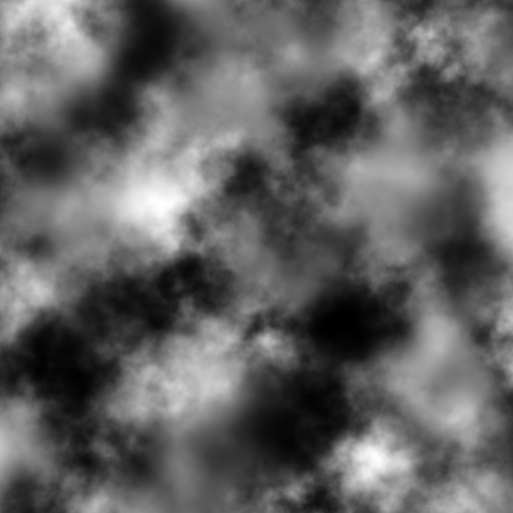
\includegraphics[width=4cm]{Ogre/Base_de_Ogre/Garder_les_pieds_sur_terre/images/terrain.png} %l'image est retaill\'ee pour avoir une largeur de 10cm
\end{figure}

Comme vous le voyez c'est une simple image en noir et blanc, et pourtant cela suffit amplement !

En effet, si l'on utilise uniquement des niveaux de gris dans une image, chaque pixel peut prendre 256 valeurs, 0 correspondant au noir et \`a la hauteur la plus faible, 255 au blanc et \`a la plus forte altitude. On a donc 256 altitudes possibles pour notre terrain, ce qui est tout \`a fait honn\^ete et suffit \`a la majorit\'e des cas.

En r\'ealit\'e, chaque pixel poss\`ede trois valeurs, correspondant \`a la quantit\'e de rouge, de vert et de bleu, chacune de ces valeurs allant de 0 \`a 255. Or pour les niveaux de gris, ces trois valeurs doivent \^etre identiques, ce qui laisse 255 triplets de valeurs : (0, 0, 0) pour le noir, puis les niveaux de gris et enfin (255, 255, 255) pour le blanc).

Lors de la cr\'eation d'un fichier heightmap, on fait en sorte que le point le plus haut de notre carte soit blanc et que le point le plus bas soit noir, afin d'utiliser toute la plage de valeurs disponibles dans la carte et \'eviter les d\'enivellations peu naturelles.

Pour charger un fichier heightmap, on passe par un objet Image qui va chercher le nom du fichier que vous voulez dans les ressources d\'ej\`a charg\'ees. J'utilise le fichier terrain.png, que vous pouvez trouver dans ''media/materials/textures''.

\begin{lstlisting}[caption={Chargement du fichier heightmap}]
Ogre::Image img;
img.load(''terrain.png'', Ogre::ResourceGroupManager::DEFAULT_RESOURCE_GROUP_NAME);
\end{lstlisting}






\subsubsection{Les param\`etres g\'eom\'etriques}


Pour fournir toutes les informations dont le terrain a besoin pour \^etre g\'en\'er\'e, on utilise sa m\'ethode prepare()\index{prepare()}\index{Terrain!prepare()} qui prend en param\`etre un Terrain::ImportData\index{ImportData}\index{Terrain!ImportData}, qui est en gros une classe contenant l'ensemble des param\`etres \`a fournir au terrain. On va donc commencer par cr\'eer cet objet :

\begin{lstlisting}[caption={Cr\'eation de l'objet ImportData pour la d\'efinition des param\`etres \`a fournir au terrain}]
Ogre::Terrain::ImportData imp;
imp.inputImage = &img;  //recuperation de l'image
imp.terrainSize = img.getWidth();  //recuperation de la taille de l'image
imp.worldSize = 8000;  //indique la taille du terrain
imp.inputScale = 600;  //echelle adoptee pour l'altitude du terrain
imp.minBatchSize = 33; //taille min du batch pour le terrain
imp.maxBatchSize = 65; //taille max du batch pour le terrain
\end{lstlisting}

On commence par r\'ecup\'erer l'image et sa taille avec les lignes 2 et 3. \textbf{\'Etant donn\'e que les terrains sont carr\'es, votre image doit elle aussi \^etre carr\'ee}, faites attention \`a cela.

Ensuite, le param\`etre worldSize\index{worldSize}\index{Terrain!worldSize} indique la taille du terrain, c'est-\`a-dire la longueur de ses c\^ot\'es en unit\'es de la sc\`ene. Plus ce nombre est grand, plus l'image est agrandie.

inputScale\index{inputScale}\index{Terrain!inputScale} correspond \`a l'\'echelle adopt\'ee pour l'altitude du terrain. C'est la hauteur qui s\'epare un point de la carte repr\'esent\'e par un pixel noir d'un point repr\'esent\'e par un pixel blanc. Il doit donc \^etre choisi en parall\`ele avec la taille du monde, puisque s'il est trop \'elev\'e et que le monde est trop petit, vous aurez un relief tr\`es escarp\'e.

Les deux derni\`eres valeurs minBatchSize \index{minBatchSize}\index{Terrain!minBatchSize} et maxBatchSize \index{maxBatchSize}\index{Terrain!maxBatchSize} renseignent les tailles minimale et maximale de batch pour notre terrain.



\subsubsection{La Batch Size\index{Batch Size}\index{Terrain!Batch}}


Le mot anglais batch signifie ''lot'' ou ''paquet''. L'affichage de mod\`ele 3D \`a l'\'ecran consommant beaucoup de ressources, plut\^ot que de chercher \`a calculer dans les moindres d\'etails la fa\c{c}on dont appara\^it la pelouse \`a l'autre bout du paysage, pour ensuite ne l'afficher que sur une toute petite surface de l'\'ecran, le moteur va simplifier les choses et calculer de fa\c{c}on grossi\`ere l'affichage de ces objets.

Ainsi, les textures peuvent \^etre simplifi\'ees, mais aussi les meshs, dont l'ordinateur va r\'eduire le nombre de vertices pour avoir moins de calculs \`a faire, vu que vous ne voyez pas les d\'etails (on parle aussi de niveau de d\'etail\index{niveau de d\'etail}, ou LOD\index{LOD}).

Pour un terrain, le maillage pourrait donc avoir un aspect similaire \`a celui-ci (image issue du wiki d'Ogre3D.org) :
Image utilisateur

Le terrain est divis\'e en lots dont la taille varie en fonction de la distance de la cam\'era \`a ces lots. Plus on s'\'eloigne, plus le lot est simplifi\'e par suppression de vertices. Lorsque plusieurs lots atteignent une taille minimale, ils sont regroup\'es en un seul lot, qui est \`a son tour simplifi\'e progressivement si la cam\'era continue de reculer.

La zone o\`u se situe la cam\'era est la plus d\'etaill\'ee, le reste est simplifi\'e.

Si la taille minimum de batch est faible, les lots adjacents auront plus facilement un niveau de d\'etail \'equivalent, mais il y aura plus de lots \`a g\'erer par l'ordinateur. En revanche, si elle est \'elev\'ee, on regroupe plus rapidement les lots, mais les fronti\`eres entre ceux-ci sont plus facilement visibles, car le niveau de d\'etail peut varier plus fortement.

Les valeurs que j'ai mises sont des valeurs courantes, sachez juste que la taille maximum est de 65 et qu'\textbf{elles doivent ob\'eir \`a la formule suivante :
taille=2n+1}



\subsubsection{Mise en place des textures\index{texture}\index{Terrain!texture}}

Pour g\'erer les textures, l'outil Terrain d'Ogre utilise des calques\index{calque}\index{Terrain!calque}. Chacun de ces calques correspond \`a une texture, que vous pourrez ensuite appliquer o\`u bon vous semblera.

Comme on parle de calques, autant vous dire tout de suite qu'il est possible de les superposer, de donner plus ou moins d'intensit\'e \`a un calque, pour cr\'eer des effets \'elabor\'es.

Nous allons commencer avec une seule texture pour faire simple et assimiler le principe. Tout se fait \`a l'aide de notre importateur de donn\'ees :

\begin{lstlisting}[caption={Mise en place d'une texture pour le terrain}]
//donne la taille de la liste de calques
imp.layerList.resize(1);

//donne la taille de la texture dans le monde
imp.layerList[0].worldSize = 100;  

//les deux lignes suivantes inserent chacune une texture dans notre calque
imp.layerList[0].textureNames.push\_back(''grass\_green-01\_diffusespecular.dds'');
imp.layerList[0].textureNames.push\_back(''grass\_green-01\_normalheight.dds'');
\end{lstlisting}

Ici les fonctions sont relativement explicites.

La premi\`ere ligne donne la taille de la liste de calques, ici je n'en ai mis qu'un seul. La seconde ligne donne la taille de la texture dans le monde. \textbf{Plus le nombre\footnote{ce nombre est-il le nombre affect\'e \`a la taille de la texture?} est important, plus la texture sera zoom\'ee, et inversement.}

Les deux lignes suivantes ins\`erent chacune une texture dans notre calque (textureNames est un vector).

Deux textures ? Je croyais qu'on mettait les textures sur des calques diff\'erents ?

En fait, on devrait plut\^ot dire qu'un calque contient un mat\'eriau\index{mat\'eriau}.

Les mat\'eriaux sont faits avec deux textures :

\begin{itemize}
\item une texture diffuse, qui contient les couleurs, les motifs du mat\'eriau ;
\item une texture normale, contenant des informations sur le relief du mat\'eriau.
\end{itemize}
   

La combinaison de ces deux textures permet d'avoir un mat\'eriau complet.



\subsubsection{Filtrage anisotrope\index{Filtrage anisotrope}\index{Terrain!Filtrage anisotrope}}


Je vais revenir rapidement sur le niveau de d\'etail\index{niveau de d\'etail}\index{Terrain!niveau de d\'etail}, qui est r\'eglable pour les mat\'eriaux via le filtrage de texture.

Vous pouvez r\'egler la nettet\'e du placage de textures sur vos meshs via un niveau de filtrage\index{niveau de filtrage}\index{Terrain!niveau de filtrage}.

On peut distinguer quatre options de filtrages, de la plus grossi\`ere \`a la plus pr\'ecise :

\begin{itemize}
\item aucun filtrage ;
\item bilin\'eaire\index{niveau de filtrage!bilin\'eaire} ;
\item trilin\'eaire\index{niveau de filtrage!trilin\'eaire} ;
\item anisotrope\index{niveau de filtrage!anisotrope}.
\end{itemize}


Voici la diff\'erence entre un filtrage anisotrope (\`a gauche) et une texture sans filtrage (\`a droite). La diff\'erence est relativement subtile ici mais visible tout de m\^eme.

Image utilisateur

Je vous propose donc d'opter pour un filtrage anisotrope, avec une valeur de 8 (la valeur par d\'efaut est 1 et \'equivaut \`a l'absence de filtrage). Vous devez donc rajouter ces deux lignes dans votre code, au d\'ebut de la m\'ethode createScene() par exemple.

\begin{lstlisting}[caption={Choix d'un filtrage anisotrope}]
Ogre::MaterialManager::getSingleton().setDefaultTextureFiltering(Ogre::TFO\_ANISOTROPIC);
Ogre::MaterialManager::getSingleton().setDefaultAnisotropy(8);
\end{lstlisting}

Le filtrage de textures n'est pas propre uniquement aux terrains, mais affecte toutes les textures affich\'ees par le moteur.


\subsubsection{Chargement et nettoyage}


Une fois que les param\`etres ont \'et\'e d\'efinis dans l'ImportData, il ne reste qu'\`a pr\'eparer et charger le terrain :

\begin{lstlisting}[caption={Pr\'eparation et chargement du terrain}]
mTerrain->prepare(imp);
mTerrain->load();
\end{lstlisting}

Pour terminer et faire un peu de place en m\'emoire, il est conseill\'e d'appeler la m\'ethode suivante qui se chargera de lib\'erer la m\'emoire allou\'ee temporairement pour la cr\'eation de votre terrain. Placez donc cette ligne \`a la fin de la m\'ethode createTerrain().

\begin{lstlisting}[caption={Lib\'eration de place en m\'emoire}]
mTerrain->freeTemporaryResources();
\end{lstlisting}

Compilez et lancez l'application pour obtenir un joli paysage !
































%---------------------------------------------------------------------------------------------------------------


\section{Le plaquage de textures}


Ogre nous permet d'utiliser diff\'erents calques pour nos mat\'eriaux. On va pouvoir mettre les calques les uns sur les autres, modifier leur opacit\'e pour avoir une texture plus ou moins visible, tout en d\'ecidant de la zone o\`u l'on veut appliquer la texture.

La premi\`ere \'etape consiste \`a rajouter des calques dans notre liste, avant de cr\'eer le terrain. Remplacez le bloc que vous aviez par le code suivant, afin d'ajouter deux nouveaux mat\'eriaux.



\begin{lstlisting}[caption={Ajout de calques}]
imp.layerList.resize(3);

imp.layerList[0].worldSize = 100;
imp.layerList[0].textureNames.push_back("grass_green-01_diffusespecular.dds");
imp.layerList[0].textureNames.push_back("grass_green-01_normalheight.dds");

imp.layerList[1].worldSize = 30;
imp.layerList[1].textureNames.push_back("growth_weirdfungus-03_diffusespecular.dds");
imp.layerList[1].textureNames.push_back("growth_weirdfungus-03_normalheight.dds");

imp.layerList[2].worldSize = 200;
imp.layerList[2].textureNames.push_back("dirt_grayrocky_diffusespecular.dds");
imp.layerList[2].textureNames.push_back("dirt_grayrocky_normalheight.dds");

mTerrain->prepare(imp);
mTerrain->load();
\end{lstlisting}

Par d\'efaut, c'est uniquement le premier mat\'eriau qui est affich\'e donc si vous ex\'ecutez le code maintenant, rien n'aura chang\'e sur votre terrain.  Il est donc n\'ecessaire d'ajouter quelques lignes pour dire de quelle fa\c{c}on nous voulons faire notre plaquage de texture.\newline

Le principe est simple \`a comprendre, chaque calque d'un terrain poss\`ede un objet TerrainLayerBlendMap\index{TerrainLayerBlendMap}\index{Terrain!TerrainLayerBlendMap} (que j'appellerai dor\'enavant Blend Map\index{Blend Map}) qui exprime la fa\c{c}on dont le calque est fusionn\'e avec les calques inf\'erieurs (le calque le plus bas est le calque 0).

Cette fusion\index{fusion de calques}\index{Terrain!fusion de calques} est simplement une affaire de transparence. Les calques sont plac\'es les uns sur les autres, et la composante transparente indique si la texture en dessous est plus ou moins visible. Il est de plus possible de faire varier la transparence du calque en chaque point de celui-ci, ce qui permet d'avoir un placage par zone.\newline

\`A la suite du bloc de code pr\'ec\'edent, commencez par r\'ecup\'erer les Blend Map correspondant au calque num\'ero 1, que nous venons d'ajouter (nous nous occuperons du second ensuite).

\begin{lstlisting}[caption={R\'ecup\'eration du Blend Map pour le premier terrain}]
Ogre::TerrainLayerBlendMap* blendMap1 = mTerrain->getLayerBlendMap(1);
\end{lstlisting}

Nous allons commencer par plaquer une seule texture au-dessus de l'herbe, sur toute la surface de notre terrain.

L'id\'ee est de parcourir l'ensemble des points du calque avec deux boucles for (il y a autant de points qu'il y avait de pixels dans notre heightmap) et de leur attribuer la transparence d\'esir\'ee, entre 1 (totalement opaque) et 255 (transparent).

La valeur la plus faible est bien 1 et non 0. Si vous mettez 0, la texture est transparente !

\begin{lstlisting}[caption={Attribution de la transparence d\'esir\'ee sur tous les points du calque}]
float* pBlend1 = blendMap1->getBlendPointer();

for (Ogre::uint16 y = 0; y < mTerrain->getLayerBlendMapSize(); ++y)
{
    for (Ogre::uint16 x = 0; x < mTerrain->getLayerBlendMapSize(); ++x)
    {   
        // opacite desiree pour le point courant
        *pBlend1++ = 150;
    }
}
\end{lstlisting}















Pour terminer, il faut mettre \`a jour notre Blend Map en appelant les m\'ethodes dirty()\index{dirty()}\index{Blend Map!dirty()} puis update()\index{update()}\index{Blend Map!update()}. La premi\`ere sert \`a pr\'eciser que les donn\'ees de la Blend map sont obsol\`etes et doivent \^etre mises \`a jour, tandis que la seconde fait effectivement la mise \`a jour.

Si vous n'appelez pas d'abord dirty(), update() n'aura aucun effet.

\begin{lstlisting}[caption={Mise \`a jour de la Blend Map}]
blendMap1->dirty();
blendMap1->update();
\end{lstlisting}

Je vous mets le code complet de la m\'ethode createTerrain() si vous voulez v\'erifier que tout est en ordre :

\begin{lstlisting}[caption={createTerrain (code complet)}]
mTerrain = OGRE_NEW Ogre::Terrain(mSceneMgr);

// options globales
mGlobals = OGRE_NEW Ogre::TerrainGlobalOptions();
mGlobals->setMaxPixelError(10);
mGlobals->setCompositeMapDistance(8000);
mGlobals->setLightMapDirection(mLight->getDerivedDirection());
Globals->setCompositeMapAmbient(mSceneMgr->getAmbientLight());
mGlobals->setCompositeMapDiffuse(mLight->getDiffuseColour());
Ogre::Image img;
img.load("terrain.png", Ogre::ResourceGroupManager::DEFAULT_RESOURCE_GROUP_NAME);

// informations g\'eom\'etriques
Ogre::Terrain::ImportData imp;
imp.inputImage = &img;
imp.terrainSize = img.getWidth();
imp.worldSize = 8000;
imp.inputScale = 600;
imp.minBatchSize = 33;
imp.maxBatchSize = 65;

// textures
imp.layerList.resize(3);
imp.layerList[0].worldSize = 100;
imp.layerList[0].textureNames.push_back("grass_green-01_diffusespecular.dds");
imp.layerList[0].textureNames.push_back("grass_green-01_normalheight.dds");
imp.layerList[1].worldSize = 30;
imp.layerList[1].textureNames.push_back("growth_weirdfungus-03_diffusespecular.dds");
imp.layerList[1].textureNames.push_back("growth_weirdfungus-03_normalheight.dds");
imp.layerList[2].worldSize = 200;
imp.layerList[2].textureNames.push_back("dirt_grayrocky_diffusespecular.dds");
imp.layerList[2].textureNames.push_back("dirt_grayrocky_normalheight.dds");
mTerrain->prepare(imp);35mTerrain->load();

// plaquage de texture
Ogre::TerrainLayerBlendMap* blendMap1 = mTerrain->getLayerBlendMap(1);
float* pBlend1 = blendMap1->getBlendPointer();
for (Ogre::uint16 y = 0; y < mTerrain->getLayerBlendMapSize(); ++y)
{
    for (Ogre::uint16 x = 0; x < mTerrain->getLayerBlendMapSize(); ++x)
    {
        *pBlend1++ = 150;
    }
}

blendMap1->dirty();
blendMap1->update();

mTerrain->freeTemporaryResources();
\end{lstlisting}

Vous pouvez maintenant ex\'ecuter l'application ! Profitez-en pour v\'erifier en vous approchant du sol que l'on distingue bien l'herbe et par-dessus la terre.
Image utilisateur

On va tout de suite essayer de faire quelque chose de plus esth\'etique.

Pour cela, maintenant que vous avez saisi les grandes \'etapes, je vous propose un mini-TP pour vous entra\^iner.








\subsection{Au boulot !}



\subsubsection{Objectif}

Une image vaut s\^urement mieux qu'un long discours, voici donc ce que vous allez devoir obtenir :
Image utilisateur

L'id\'ee est de texturer le terrain en fonction de l'altitude. Si l'on est en dessous d'un certain seuil, il n'y a que de la terre qui appara\^it ; au-dessus, on a de l'herbe.



\subsubsection{Indications}

Je vous donne tout de m\^eme les m\'ethodes qui sont utiles, notamment pour trouver l'altitude du terrain en fonction de la position :

\begin{lstlisting}[caption={m\'ethode getHeightAtTerrainPosition pour trouver l'altitude du terrain en fonction de la position }]
float Ogre::Terrain::getHeightAtTerrainPosition(Ogre::Real x, Ogre::Real y)
\end{lstlisting}

Cette fonction retourne l'altitude en fonction de la position, sachant que x et y sont compris entre 0 et 1.

Pour r\'ecup\'erer ces deux valeurs, on utilise une m\'ethode de TerrainLayerBlendMap qui convertit les coordonn\'ees de l'image en coordonn\'ees du terrain (celles dont vous avez besoin) :

\begin{lstlisting}[caption={M\'ethode convertImageToTerrainSpace pour convertir les coordonn\'ees de l'image en coordonn\'ees du terrain}]
void Ogre::TerrainLayerBlendMap::convertImageToTerrainSpace(size_t x, size_t y, Ogre::Real * outX, Ogre::Real * outY)
\end{lstlisting}


Enfin, je vous laisse choisir l'altitude limite entre l'herbe et la terre. Vous avez toutes les cartes en mains maintenant.

























\subsubsection{Correction}

Comme avez d\^u le deviner, tout se passe dans les deux boucles for.

Pour chaque point parcouru, on recherche ses coordonn\'ees dans le rep\`ere du terrain, puis on r\'ecup\`ere la hauteur, que l'on compare \`a notre hauteur limite. Si on est en dessous, on affiche la texture de terre avec une opacit\'e maximum, sinon on ne fait qu'incr\'ementer le pointeur de la Blend map.

Voici donc le code modifi\'e :

\begin{lstlisting}[caption={Attribution de la transparence d\'esir\'ee sur tous les points du calque selon leur position}]
for (Ogre::uint16 y = 0; y < mTerrain->getLayerBlendMapSize(); ++y)
{
    for (Ogre::uint16 x = 0; x < mTerrain->getLayerBlendMapSize(); ++x)
    {
        Ogre::Real terrainX, terrainY;
        blendMap1->convertImageToTerrainSpace(x, y, &terrainX, &terrainY);
        Ogre::Real height = mTerrain->getHeightAtTerrainPosition(terrainX, terrainY);
        if(height < 200)
            *pBlend1 = 1;
        pBlend1++;
    }
}
\end{lstlisting}

Vous pouvez aussi bien s\^ur r\'ecup\'erer la Blend map num\'ero 2 plus haut pour voir le r\'esultat avec une autre texture, c'est ce que j'ai fait pour obtenir l'image r\'ef\'erence pour le TP.








\subsubsection{Code}

Ci-dessous le trouve le code de la metohde createTerrain et le resultat obtenu:

\begin{lstlisting}[caption={createTerrain}]
void PremiereApplication::createTerrain()
{    
    Ogre::Vector3 lightdir(0.55f, -0.3f, 0.75f);
    
    mLight = mSceneMgr->createLight("terrainLight");
    mLight->setType(Light::LT_DIRECTIONAL);
    mLight->setDirection(lightdir);
    mLight->setDiffuseColour(Ogre::ColourValue::White);
    mLight->setSpecularColour(Ogre::ColourValue(0.4f, 0.4f, 0.4f)); 
    
    mGlobals = OGRE_NEW Ogre::TerrainGlobalOptions();
    mGlobals->setMaxPixelError(8);                                      /**<spécifie la précision de rendu (en nbr de pixel) du terrain*/    
    
    //application des réglages de lumière aux options globales
    mGlobals->setLightMapDirection(mLight->getDerivedDirection());
    mGlobals->setCompositeMapDistance(3000);
    mGlobals->setCompositeMapAmbient(mSceneMgr->getAmbientLight());
    mGlobals->setCompositeMapDiffuse(mLight->getDiffuseColour());    
    
    mTerrain = OGRE_NEW Ogre::Terrain(mSceneMgr);/**<Création du terrain*/
    
    Ogre::Image img;
    img.load("terrain.png", Ogre::ResourceGroupManager::DEFAULT_RESOURCE_GROUP_NAME);/**<Chargement de l'image Heighmaps contenant les infos pour le relief*/
    
    ///Mise en place des propriétés générales du terrain
    Ogre::Terrain::ImportData imp;/**<Création de l'objet qui contiendra toutes les infos pour le terrain*/
    imp.inputImage = &img;/**<recuperation de l image*/
    imp.terrainSize = img.getWidth();/**<recuperation de la taille de l image (les terrains sont carres, l'image doit donc etre carree)*/

    imp.worldSize = 8000;/**<taille du terrain en unites de la scene (plus ce nbre est grande, plus l'image est grande)*/
    imp.inputScale = 600;/**<echelle adoptee pour l altitude du terrain (difference entre un pt a l'altitude 0 (pt en blanc ds terrain.png) et un point à l'altitude max (pt en noir))*/
    imp.minBatchSize = 33;/**<taille min du batch pour le terrain*/
    imp.maxBatchSize = 65;/**<taille max du batch pour le terrain*/
    
    ///Mise en place des textures
    imp.layerList.resize(1);/**<donne la taille de la liste des calques*/
    imp.layerList[0].worldSize = 100;/**<donne la taille de la texture ds le monde (plus le nbre est gd plus la texture est zoomée)*/
    ///insertion de textures dans notre calque
    imp.layerList[0].textureNames.push_back("grass_green-01_diffusespecular.dds");/**>contient les couleurs, les motifs du materiau*/
    imp.layerList[0].textureNames.push_back("grass_green-01_normalheight.dds");/**<contient des infos sur le relief du materiau*/
    
    ///Filtrage anisotropique (affecte toutes les textures)
    Ogre::MaterialManager::getSingleton().setDefaultTextureFiltering(Ogre::TFO_ANISOTROPIC);
    Ogre::MaterialManager::getSingleton().setDefaultAnisotropy(8);
    
    ///Rajout de calques dans notre liste
    imp.layerList.resize(3);
    imp.layerList[0].worldSize = 100;
    imp.layerList[0].textureNames.push_back("grass_green-01_diffusespecular.dds");
    imp.layerList[0].textureNames.push_back("grass_green-01_normalheight.dds");
    imp.layerList[1].worldSize = 30;
    imp.layerList[1].textureNames.push_back("growth_weirdfungus-03_diffusespecular.dds");
    imp.layerList[1].textureNames.push_back("growth_weirdfungus-03_normalheight.dds");
    imp.layerList[2].worldSize = 200;
    imp.layerList[2].textureNames.push_back("dirt_grayrocky_diffusespecular.dds");
    imp.layerList[2].textureNames.push_back("dirt_grayrocky_normalheight.dds");
    
    mTerrain->prepare(imp);/**<on fournit toutes les informations necessaires au terrain*/
    mTerrain->load();/**<chragement du terrain*/    
    
    ///recuperation du blend map pour le premier terrain
    Ogre::TerrainLayerBlendMap* blendMap2 = mTerrain->getLayerBlendMap(2);/**<recuperation du blend map*/
    
    ///plaquage de la texture..
    float* pBlend2 = blendMap2->getBlendPointer();
    ///..en fonction de l'altitude
    for (Ogre::uint16 y = 0; y < mTerrain->getLayerBlendMapSize(); ++y)
    {
        for (Ogre::uint16 x = 0; x < mTerrain->getLayerBlendMapSize(); ++x)
        {
            Ogre::Real terrainX, terrainY;
            
            blendMap2->convertImageToTerrainSpace(x, y, &terrainX, &terrainY);
            Ogre::Real height = mTerrain->getHeightAtTerrainPosition(terrainX, terrainY);
            
            //en general l'herbe se trouve en basse altitude
            if(height > 200)
                *pBlend2 = 1;
            
            pBlend2++;
        }
    }
    
    blendMap2->dirty();/**<precise que les donnees de la blend Map st obsolètes*/
    blendMap2->update();/**<fait la mise a jour des donnees de la blend map*/ 
    
    mTerrain->freeTemporaryResources();/**<liberation de la memoire allouee temporairement*/
}

\end{lstlisting}




\begin{lstlisting}[caption={PremiereApplication.h}]

using namespace std;

#include <ExampleApplication.h>
#include <OgreMovableObject.h>
#include "InputListener.h"

#include <Terrain/OgreTerrain.h>

class PremiereApplication : public ExampleApplication
{    
    public:
        Terrain *mTerrain;                      /**<gèrera les propriétés de notre terrain*/
        Ogre::TerrainGlobalOptions *mGlobals;   /**<objet obligatoire pr la gestion des terrains, définira les propriétés générales pour le terrain (ex: éclairage)*/
        Light *mLight;                          /**<contiendra les proriétés de la lumière*/
        
        /** Crée la scène avec une tête d'Ogre flottant sur un carré de pelouse
         */
        void createScene();
        
        /** Crée et place la caméra
         */
        void createCamera();
        
        /** Crée une seconde vue de la scene
         */
        void createViewports();

        /** Gère les entrées 
         */
        void createFrameListener();
        
        /** Crée une lumière selon le paramètre
         @param luxType - type de lumière désirée 
         @param lux - instance de lumière 
         @return distance to point
         */
        //void createLux(std::string luxType, MovableObject *lux);
        
        /** Initialise le terrain
         */
        void createTerrain();
};
\end{lstlisting}













\begin{lstlisting}[caption={CMakeLists.txt}]
project(helloworld)
cmake_minimum_required(VERSION 2.6)

set(CMAKE_MODULE_PATH "/usr/share/OGRE/cmake/modules")

set(CMAKE_CXX_FLAGS "-Wall -std=c++11 -g")

# Il s'agit du tutoriel d'exemple, qui utilise quelques fichiers prdfini de Ogre. Il faut indiquer a cmake ou se trouvent les includes en question
include_directories ("include")

# Bien sur, pour compiler Ogre, il faut le chercher, et dfinir le rpertoire contenant les includes.
find_package(OGRE REQUIRED)
include_directories (${OGRE_INCLUDE_DIRS})

if (OGRE_Overlay_FOUND)
# append OgreOverlay to the end of the OGRE_LIBRARIES variable
  set(OGRE_LIBRARIES ${OGRE_LIBRARIES} ${OGRE_Overlay_LIBRARIES})
  message(STATUS "Found OGRE_Terrain: ${OGRE_Overlay_LIBRARIES}")
else (OGRE_Overlay_FOUND)
  message(SEND_ERROR "OgreOverlay Library not found.")
endif(OGRE_Overlay_FOUND)

#Inclusion de la lib libOgreTerrain.so
if (OGRE_Terrain_FOUND)
  set(OGRE_LIBRARIES ${OGRE_LIBRARIES} ${OGRE_Terrain_LIBRARIES})
  message(STATUS "Found OGRE_Terrain: ${OGRE_Terrain_LIBRARIES}")
else (OGRE_Terrain_FOUND)
  message(SEND_ERROR "OgreTerrain Library not found.")
endif(OGRE_Terrain_FOUND)


#Inclusion de la lib libOgrePaging.so
if (OGRE_Paging_FOUND)
  set(OGRE_LIBRARIES ${OGRE_LIBRARIES} ${OGRE_Paging_LIBRARIES})
  message(STATUS "Found OGRE_Paging: ${OGRE_Paging_LIBRARIES}")
else (OGRE_Paging_FOUND)
  message(SEND_ERROR "OgrePaging Library not found.")
endif(OGRE_Paging_FOUND)


# L'exemple depend aussi de OIS, une lib pour gerer la souris, clavier, joystick...
find_package(OIS REQUIRED)

# On dfinit les sources qu'on veut compiler
SET( SOURCES
  src/InputListener.cpp  
  src/PremiereApplication.cpp
  src/main.cpp
)

# On les compile
add_executable (
  premiereapp ${SOURCES}
)

message(STATUS "OGRE Libraries used to link are ${OGRE_LIBRARIES}")

# Et pour finir, on lie l'executable avec les librairies que find_package nous a gentillement trouve.
target_link_libraries(premiereapp ${OGRE_LIBRARIES} ${OIS_LIBRARY} -lboost_system)



set( RESOURCES_FILE
  media/
  resources/ogre.cfg
  resources/plugins.cfg
  resources/resources.cfg
)

# do the copying
foreach( file_i ${RESOURCES_FILE})
    add_custom_command(
      TARGET premiereapp
      POST_BUILD
      COMMAND cp -R ${CMAKE_SOURCE_DIR}/${file_i} ${CMAKE_BINARY_DIR}
      COMMENT "copy file ${file_i}"
      )
endforeach( file_i )

\end{lstlisting}





Et on obtiend:
\begin{figure}[hbtp]
\caption{Terrain.png}
\centering
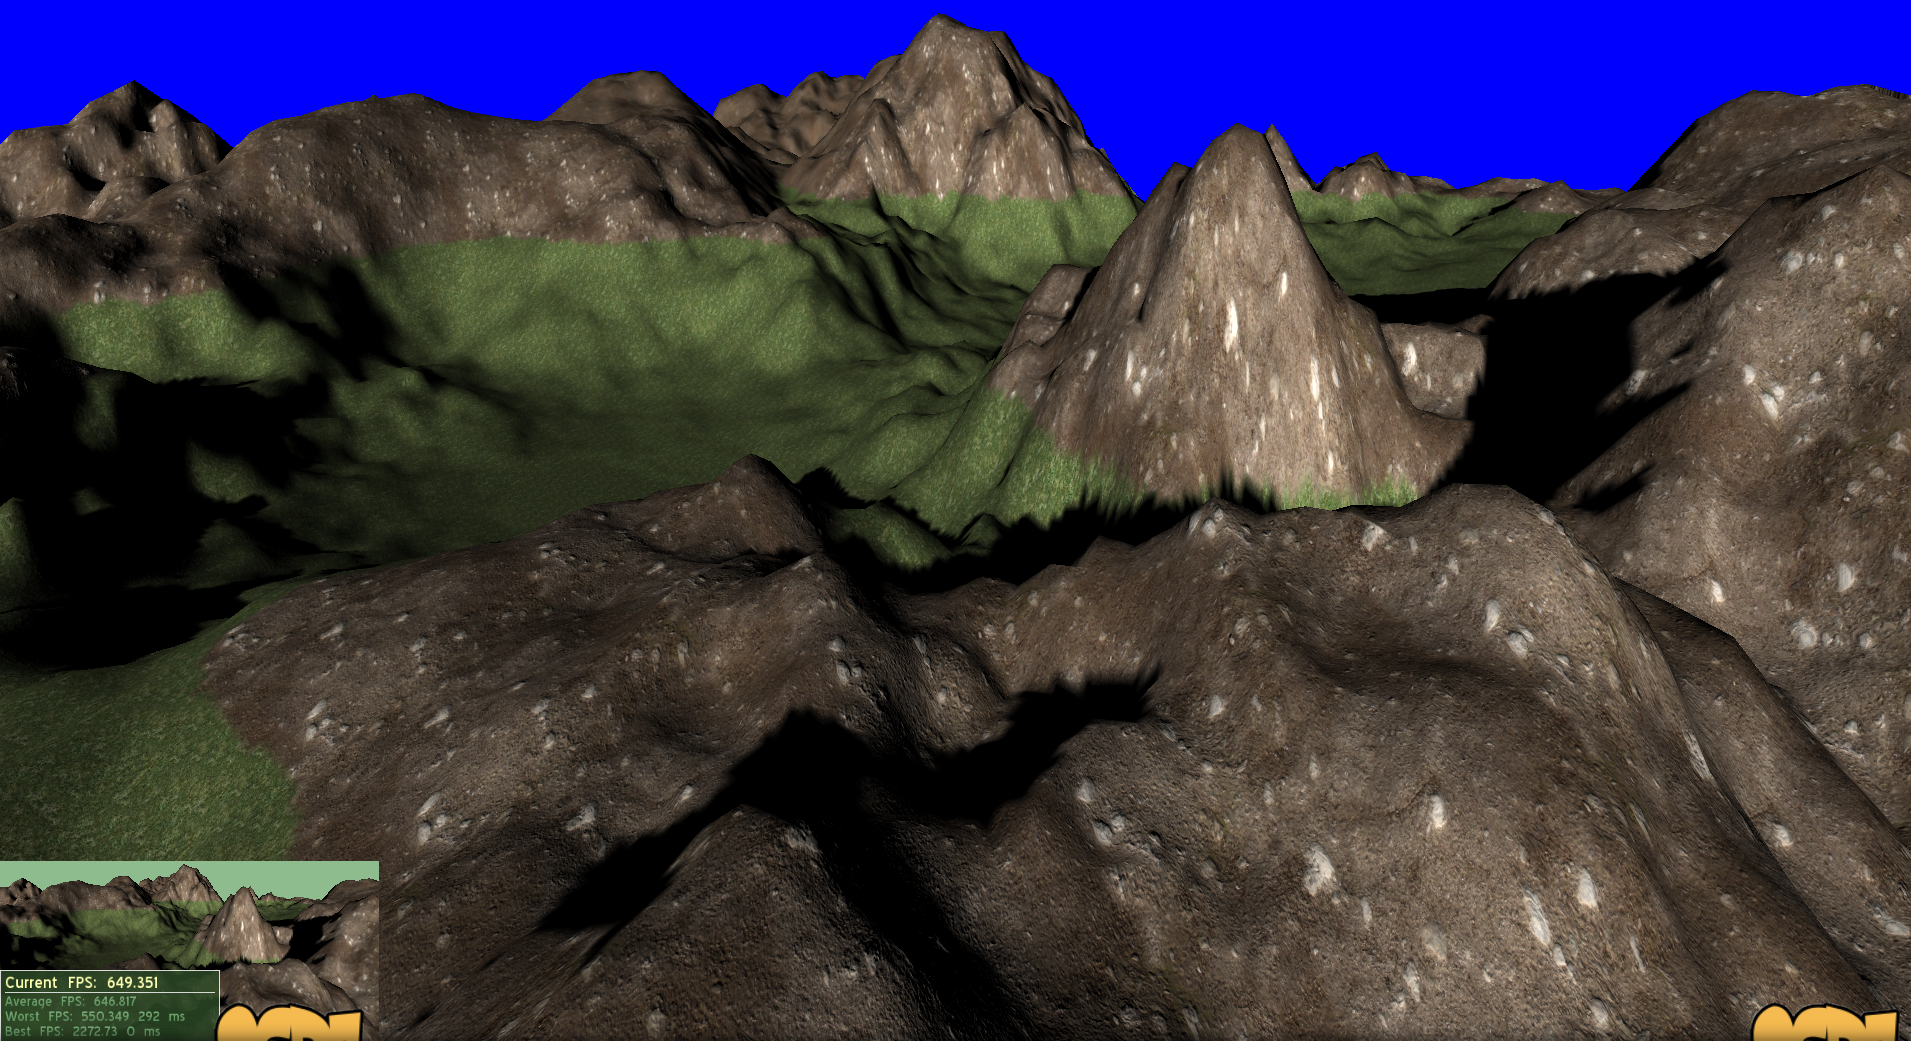
\includegraphics[width=8cm]{Ogre/Base_de_Ogre/Garder_les_pieds_sur_terre/images/Differentes_textures_selon_altitude1.png} %l'image est retaill\'ee pour avoir une largeur de 10cm
\end{figure}




















\subsection{Pour aller plus loin}


Sur le m\^eme principe, nous allons voir comment appliquer deux textures diff\'erentes sur une petite largeur, \`a une altitude donn\'ee.

Ceci peut \^etre utile si vous voulez r\'ealiser des \'etendues d'eau dans votre terrain : au bord de l'eau, il y a de la boue, un peu au-dessus, de la terre s\`eche, puis ensuite l'herbe reprend ses droits. C'est ce que nous allons faire, avec une opacit\'e progressive, mais sans l'eau, ce sera pour plus tard.

Nous devons commencer par r\'ecup\'erer un pointeur sur notre seconde Blend Map pour pouvoir g\'erer la seconde texture en plus de la premi\`ere. Il y a donc deux lignes \`a rajouter en cons\'equence avant les boucles.




\begin{lstlisting}[caption={R\'ecup\'eration des Blend Map pour le premier et le second terrain}]
Ogre::TerrainLayerBlendMap* blendMap1 = mTerrain->getLayerBlendMap(1);
Ogre::TerrainLayerBlendMap* blendMap2 = mTerrain->getLayerBlendMap(2);

float* pBlend1 = blendMap1->getBlendPointer();
float* pBlend2 = blendMap2->getBlendPointer();
\end{lstlisting}

D\'efinissons aussi deux variables pour chacune des textures : la hauteur \`a laquelle se situe la texture et la largeur de la bande que l'on veut obtenir.

\begin{lstlisting}[caption={}]
Ogre::Real minHeight1 = 70;
Ogre::Real fadeDist1 = 40;
Ogre::Real minHeight2 = 70;
Ogre::Real fadeDist2 = 15;
\end{lstlisting}

Dans la boucle, on d\'eclare trois variables : deux coordonn\'ees du terrain et la transparence pour le point actuel.

\begin{lstlisting}[caption={}]
Ogre::Real terrainX, terrainY, transparence;
\end{lstlisting}

On r\'ecup\`ere ensuite la hauteur du terrain comme pr\'ec\'edemment.

\begin{lstlisting}[caption={}]
blendMap1->convertImageToTerrainSpace(x, y, &terrainX, &terrainY);
Ogre::Real height = mTerrain->getHeightAtTerrainPosition(terrainX, terrainY);
\end{lstlisting}

Ensuite, pour chaque texture, on calcule la diff\'erence entre la hauteur du point actuel et la hauteur que l'on veut pour la texture, divis\'ee par la largeur de la bande. Si le point est cens\'e \^etre recouvert par la texture, ce nombre sera donc compris entre 0 et 1.

On utilise ensuite la m\'ethode statique Clamp() qui a pour prototype :

\begin{lstlisting}[caption={Utilisation de la m\'ethode statique Clamp()}]
static T Ogre::Math::Clamp(T val, T minval, T maxval)
\end{lstlisting}

Si val est inf\'erieure \`a minval, la fonction retourne minval ; si val est sup\'erieure \`a maxval, on retourne maxval. Si val est dans l'intervalle, on la retourne directement.

Comme on ne veut afficher que les points dont la valeur calcul\'ee pr\'ec\'edemment est comprise entre 0 et 1, on va utiliser cette m\'ethode pour ''couper'' toutes les valeurs en dehors de l'intervalle.

\begin{lstlisting}[caption={}]
transparence = (height - minHeight1) / fadeDist1;
transparence = Ogre::Math::Clamp(transparence, (Ogre::Real)0, (Ogre::Real)1);
\end{lstlisting}

Pour terminer, on multiplie transparence par 255 pour avoir une valeur comprise entre 0 et 255.

\begin{lstlisting}[caption={}]
*pBlend1++ = transparence * 255;
\end{lstlisting}

On observe que si transparence est \`a l'ext\'erieur de l'intervalle [0 ; 1] apr\`es le premier calcul, Clamp retournera 0 ou 1. Quand on multiplie par 255, on obtient donc 0 ou 255, qui sont les deux valeurs pour lesquelles la texture est transparente. Mission accomplie !

On copie ces trois lignes pour la seconde texture, et on obtient le code suivant dans nos boucles :

\begin{lstlisting}[caption={}]
for (Ogre::uint16 y = 0; y < mTerrain->getLayerBlendMapSize(); ++y)
{
    for (Ogre::uint16 x = 0; x < mTerrain->getLayerBlendMapSize(); ++x)
    {
        Ogre::Real terrainX, terrainY, transparence;
        blendMap1->convertImageToTerrainSpace(x, y, &terrainX, &terrainY);
        Ogre::Real height = mTerrain->getHeightAtTerrainPosition(terrainX, terrainY);
        transparence = (height - minHeight1) / fadeDist1;
        transparence = Ogre::Math::Clamp(transparence, (Ogre::Real)0, (Ogre::Real)1);
        *pBlend1++ = transparence * 255;
        transparence = (height - minHeight2) / fadeDist2;
        transparence = Ogre::Math::Clamp(transparence, (Ogre::Real)0, (Ogre::Real)1);
        *pBlend2++ = transparence * 255;
    }
}
\end{lstlisting}

Pensez \`a mettre \`a jour la seconde Blend Map une fois que les modifications sont termin\'ees :

\begin{lstlisting}[caption={}]
blendMap1->dirty();
blendMap2->dirty();
blendMap1->update();
blendMap2->update();
\end{lstlisting}




\subsubsection{Code}
Les seules choses \`a changer sont le plaquage de texture:


\begin{lstlisting}[caption={Plaquage de textures sur zone}]
...
    ///pour definir des bandes d'altitude avec une texture différente
    Ogre::Real minHeight1 = 70;
    Ogre::Real fadeDist1 = 40;
    Ogre::Real minHeight2 = 70;
    Ogre::Real fadeDist2 = 15;
    
    
    ///recuperation du blend map pour le premier terrain
    Ogre::TerrainLayerBlendMap* blendMap1 = mTerrain->getLayerBlendMap(1);/**<recuperation du blend map*/
    Ogre::TerrainLayerBlendMap* blendMap2 = mTerrain->getLayerBlendMap(2);/**<recuperation du blend map*/
    
    ///plaquage de la texture..
    float* pBlend1 = blendMap1->getBlendPointer();
    float* pBlend2 = blendMap2->getBlendPointer();
    ///..en fonction de l'altitude
    for (Ogre::uint16 y = 0; y < mTerrain->getLayerBlendMapSize(); ++y)
    {
        for (Ogre::uint16 x = 0; x < mTerrain->getLayerBlendMapSize(); ++x)
        {
            Ogre::Real terrainX, terrainY, transparence;
            
            blendMap1->convertImageToTerrainSpace(x, y, &terrainX, &terrainY);
            Ogre::Real height = mTerrain->getHeightAtTerrainPosition(terrainX, terrainY);
            
            transparence = (height - minHeight1) / fadeDist1;
            transparence = Ogre::Math::Clamp(transparence, (Ogre::Real)0, (Ogre::Real)1);
            *pBlend1++ = transparence * 255;
            
            transparence = (height - minHeight2) / fadeDist2;
            transparence = Ogre::Math::Clamp(transparence, (Ogre::Real)0, (Ogre::Real)1);
            *pBlend2++ = transparence * 255;
        }
    }
    
    blendMap1->dirty();/**<precise que les donnees de la blend Map st obsolètes*/
    blendMap1->update();/**<fait la mise a jour des donnees de la blend map*/
    blendMap2->dirty();/**<precise que les donnees de la blend Map st obsolètes*/
    blendMap2->update();/**<fait la mise a jour des donnees de la blend map*/ 
...
\end{lstlisting}



Et on obtiend:
\begin{figure}[hbtp]
\caption{Terrain.png}
\centering
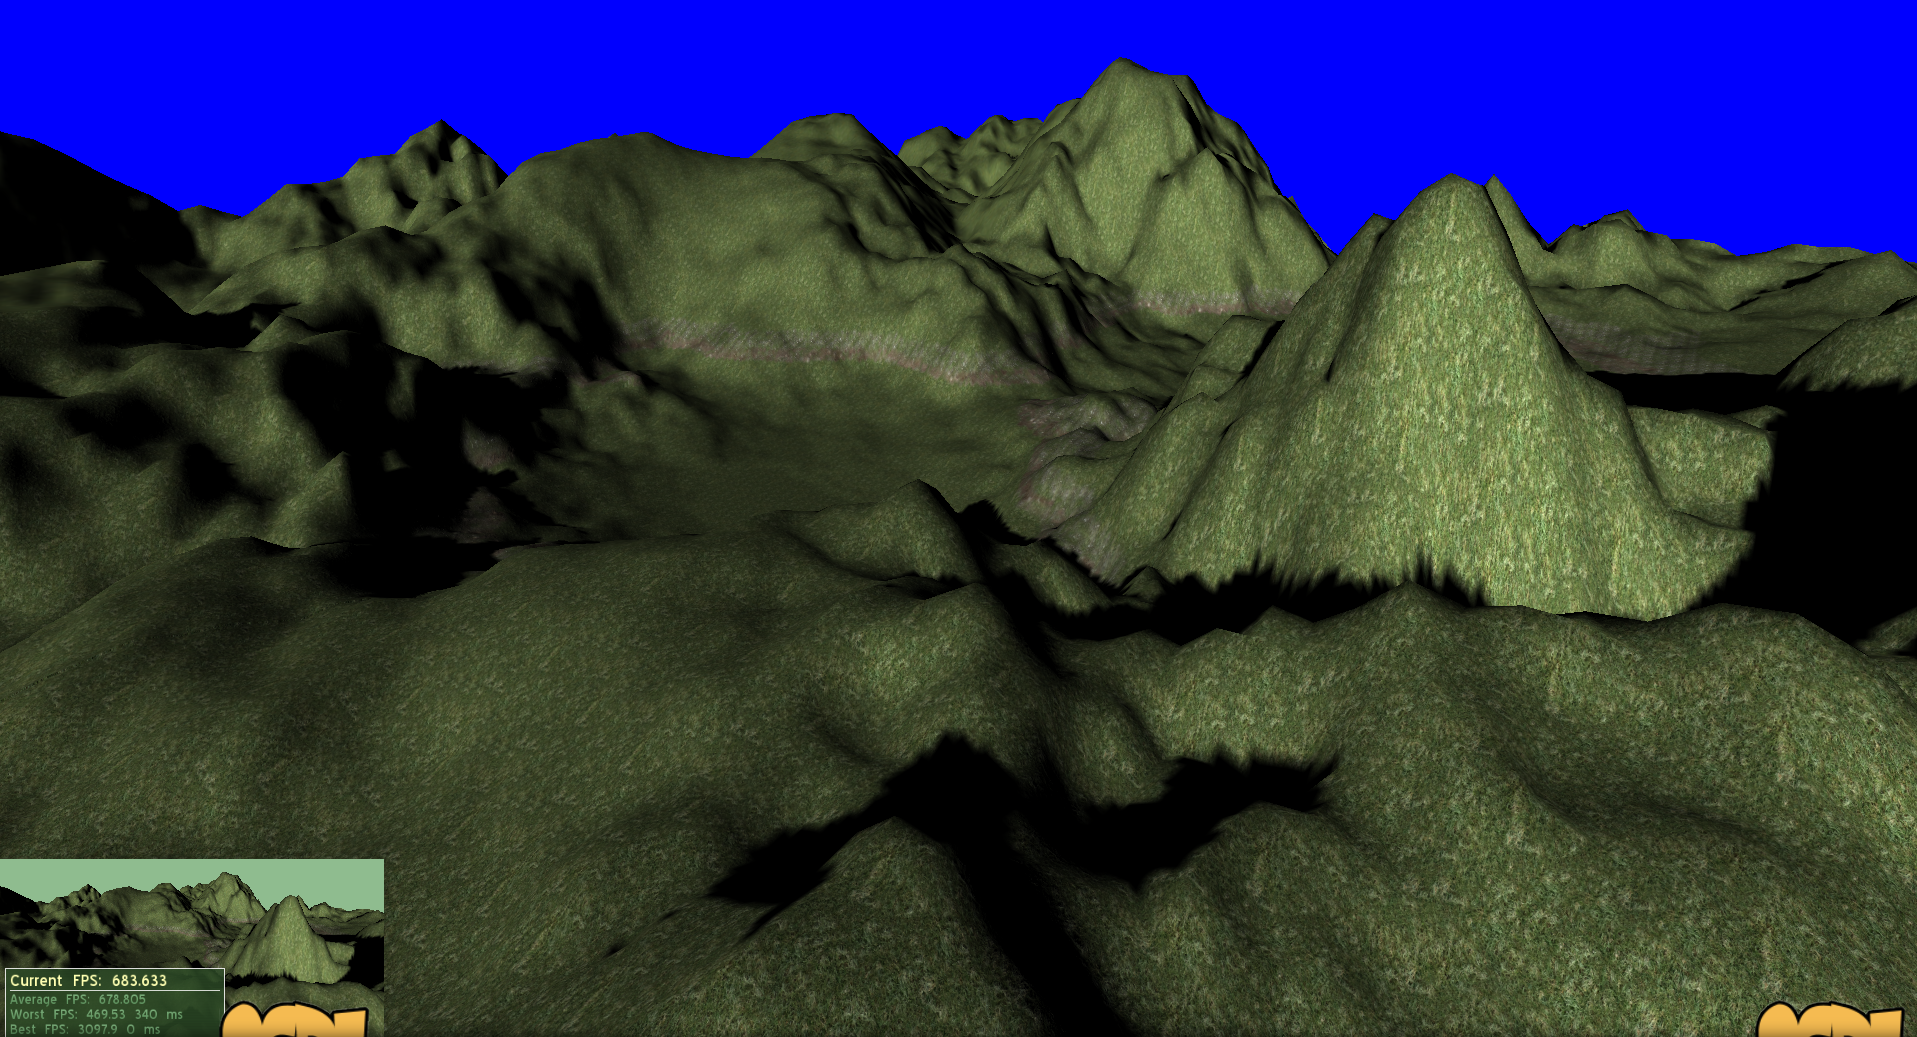
\includegraphics[width=8cm]{Ogre/Base_de_Ogre/Garder_les_pieds_sur_terre/images/Differentes_textures_selon_altitude2.png} %l'image est retaill\'ee pour avoir une largeur de 10cm
\end{figure}








%140522
%A relire, corriger et indexer à partir d ici
%---------------------------------------------------------------------------------------------------------------
\section{Les groupes de terrains}

Un groupe de terrains\index{groupe de terrains} (ou TerrainGroup\index{TerrainGroup}) range les terrains comme dans un tableau \`a deux dimensions. Dans le groupe, tous les terrains doivent avoir la m\^eme taille, afin de pouvoir les aligner dans une grille.



\subsection{Cr\'eation}

On commence par ajouter un include au d\'ebut de la classe puis on remplace notre instance de Terrain par un TerrainGroup, ensuite on l'initialisera dans notre m\'ethode createTerrain() :

\begin{lstlisting}[caption={TerrainGroup: include et cr\'eation}]
#include <Ogre/Terrain/OgreTerrainGroup.h>
//...
Ogre::TerrainGroup *mTerrainGroup;
\end{lstlisting}

Apr\`es les lignes permettant de charger l'image heightmap dans la m\'ethode createTerrain()\index{createTerrain()}, ins\'erez les lignes suivantes.

\begin{lstlisting}[caption={}]
mTerrainGroup = OGRE_NEW Ogre::TerrainGroup(mSceneMgr, Ogre::Terrain::ALIGN_X_Z, img.getWidth(), 8000);

//On definit ensuite la position de l'origine du groupe de terrains
mTerrainGroup->setOrigin(Ogre::Vector3::ZERO);

//nom (et l'extension) que l'on veut attribuer a nos fichiers qui seront crees pour sauvegarder les terrains
mTerrainGroup->setFilenameConvention(Ogre::String("TerrainDuZero"), Ogre::String("dat"));
\end{lstlisting}

Les param\`etres \`a fournir au TerrainGroup sont
\begin{itemize}
\item le Scene manager,
\item l'alignement du terrain\index{ALIGN\_X\_Z}\index{Terrain!ALIGN\_X\_Z}\index{alignement du terrain} par rapport au rep\`ere global (vous pouvez cr\'eer un terrain vertical, par exemple),
\item la taille des heightmaps utilis\'ees\index{getWidth()}\index{heightmaps!getWidth()}, 
\item la taille d'un terrain.
\end{itemize}

On d\'efinit ensuite la position de l'origine du groupe de terrains\index{setOrigin()}\index{TerrainGroup!setOrigin()}, puis le nom\index{setFilenameConvention()}\index{TerrainGroup!setFilenameConvention()} (et l'extension) que l'on veut attribuer \`a nos fichiers qui seront cr\'e\'es pour sauvegarder les terrains par la suite.

Pour les donn\'ees des terrains enregistr\'ees dans un objet ImportData, nous allons modifier un peu le fonctionnement du programme. On r\'ecup\`ere en fait directement une r\'ef\'erence sur un ImportData fourni par le TerrainGroup\index{getDefaultImportSettings()}\index{TerrainGroup!getDefaultImportSettings()}, que l'on modifie directement et qui sera valable pour l'ensemble des terrains du groupe. \`A noter que la ligne de d\'efinition de la heightmap n'est plus utile ici, cela sera indiqu\'e lors de la cr\'eation des terrains.

\begin{lstlisting}[caption={}]
Ogre::Terrain::ImportData& imp = mTerrainGroup->getDefaultImportSettings();
imp.terrainSize = img.getWidth();
imp.worldSize = 8000;
imp.inputScale = 600;
imp.minBatchSize = 33;
imp.maxBatchSize = 65;
\end{lstlisting}

Il est maintenant temps de cr\'eer les terrains du groupe. On d\'efinit la taille du groupe et pour chaque case, on appelle une m\'ethode definirTerrain() d\'efinie plus bas qui s'occupera de cr\'eer chaque terrain ind\'ependamment.

\begin{lstlisting}[caption={Cr\'eation des terrains du groupe}]
int largeur = 2, longueur = 2;

for(int x = 0; x < largeur; x++)
{
    for(int y = 0; y < longueur; y++)
    {
        definirTerrain(x, y);
    }
}
mTerrainGroup->loadAllTerrains(true);
\end{lstlisting}

Le groupe se charge pour terminer d'appeler les m\'ethodes load()\index{load()} de chaque terrain \`a travers la m\'ethode loadAllTerrains()\index{loadAllTerrains()}. Cette m\'ethode prend un bool\'een en param\`etre qui indique si le chargement doit \^etre synchrone, c'est-\`a-dire ex\'ecut\'e dans un seul thread (le thread principal ici). Par d\'efaut cette valeur est fausse, c'est-\`a-dire que les terrains sont charg\'es dans plusieurs threads si c'est possible.

Le chargement devient vite tr\`es lourd si l'on ajoute beaucoup de terrains aux groupes. Nous verrons plus bas comment acc\'el\'erer le chargement.

Maintenant, nous devons \'ecrire la m\'ethode definirTerrain() qui utilise la m\'ethode defineTerrain()\index{defineTerrain()}\index{TerrainGroup!defineTerrain()} de TerrainGroup. Celle-ci va prendre 3 param\`etres : les deux coordonn\'ees du terrain dans le groupe de terrains (sa position sur la grille, donc) et l'image heightmap utilis\'ee pour ce terrain. Les coordonn\'ees du terrain au sein du groupe peuvent \^etre n\'egatives.

Juste avant d'appeler le terrain, on va faire une v\'erification sur les coordonn\'ees : si l'abscisse du terrain est impaire, on inverse l'image suivant l'axe Y, si l'ordonn\'ee est impaire, on inverse l'image cette fois-ci selon l'axe X. Cela permet aux terrains du groupe de ne pas avoir de diff\'erence d'altitude lors des jointures. Si vous utilisez des heightmaps\index{heightmaps} diff\'erents sur les terrains du groupe (ce qui sera probablement le cas), vous devrez faire attention \`a ce que les altitudes des bords correspondent pour \'eviter les trous \`a ces endroits.

\begin{lstlisting}[caption={PremiereApplication.definirTerrain}]
void PremiereApplication::definirTerrain(int x, int y)
{
    Ogre::Image img;
    img.load("terrain.png", Ogre::ResourceGroupManager::DEFAULT_RESOURCE_GROUP_NAME);

    if(x % 2 != 0)
        img.flipAroundY();

    if(y % 2 != 0)
        img.flipAroundX();

    mTerrainGroup->defineTerrain(x, y, &img);
}
\end{lstlisting}

Une fois que les terrains sont charg\'es, il faut leur appliquer les textures d\'efinies. On utilise pour cela un it\'erateur sur le groupe de terrains et, pour chaque terrain, on appelle une m\'ethode initBlendMaps() qui contient le code pour texturer les terrains.

\begin{lstlisting}[caption={}]
Ogre::TerrainGroup::TerrainIterator ti = mTerrainGroup->getTerrainIterator();

while(ti.hasMoreElements())
{
    Ogre::Terrain* t = ti.getNext()->instance;
    initBlendMaps(t);
}
\end{lstlisting}

La m\'ethode initBlendMaps() contient uniquement du code que l'on a d\'ej\`a vu mais que j'ai d\'eplac\'e pour plus de clart\'e. Elle prend en param\`etre le terrain dont on doit modifier les Blend maps.

\begin{lstlisting}[caption={}]
void PremiereApplication::initBlendMaps(Ogre::Terrain *terrain)
{
    Ogre::TerrainLayerBlendMap* blendMap1 = terrain->getLayerBlendMap(1);
    Ogre::TerrainLayerBlendMap* blendMap2 = terrain->getLayerBlendMap(2);
    Ogre::Real minHeight1 = 70;
    Ogre::Real fadeDist1 = 40;
    Ogre::Real minHeight2 = 70;
    Ogre::Real fadeDist2 = 15;
    float* pBlend1 = blendMap1->getBlendPointer();
    float* pBlend2 = blendMap2->getBlendPointer();

    for (Ogre::uint16 y = 0; y < terrain->getLayerBlendMapSize(); ++y)
    {
        for (Ogre::uint16 x = 0; x < terrain->getLayerBlendMapSize(); ++x)
        {
            Ogre::Real terrainX, terrainY, transparence;
            blendMap1->convertImageToTerrainSpace(x, y, &terrainX, &terrainY);
            Ogre::Real height = terrain->getHeightAtTerrainPosition(terrainX, terrainY);
            transparence = (height - minHeight1) / fadeDist1;
            transparence = Ogre::Math::Clamp(transparence, (Ogre::Real)0, (Ogre::Real)1);
            *pBlend1++ = transparence * 255;
            transparence = (height - minHeight2) / fadeDist2;
            transparence = Ogre::Math::Clamp(transparence, (Ogre::Real)0, (Ogre::Real)1);
            *pBlend2++ = transparence * 255;
        }
    }
    blendMap1->dirty();
    blendMap2->dirty();
    blendMap1->update();
    blendMap2->update();
}
\end{lstlisting}

Pour terminer, comme avec un terrain seul, on lib\`ere la m\'emoire utilis\'ee par le TerrainGroup.

\begin{lstlisting}[caption={}]
mTerrainGroup->freeTemporaryResources();
\end{lstlisting}

Votre sc\`ene doit maintenant avoir une surface plus grande que la première fois (on a maintenant quatre terrains). Vous pouvez encore augmenter le nombre de terrains, mais attention, le temps de chargement augmente rapidement !



\subsection{Optimiser le temps de chargement}

Vous avez certainement remarqu\'e que la g\'en\'eration du terrain prend un temps cons\'equent lorsque le groupe s'agrandit. La cr\'eation du terrain \`a partir du fichier heightmap n\'ecessite en effet de convertir les donn\'ees de l'image en donn\'ees exploitables par le moteur.

Afin de r\'eduire le temps de chargement, il est possible d'enregistrer un fichier qui contient toutes les informations sur le terrain construit pour \'eviter de relire l'image \`a chaque lancement de l'application. L'inconv\'enient majeur est la place occup\'ee par ces fichiers g\'en\'er\'es, qui contiennent beaucoup plus d'informations qu'une simple heightmap.

En regardant la cr\'eation du groupe de terrains, vous voyez que l'on a d\'efini une convention de nommage pour des fichiers, mais qui est pour l'instant inutilis\'ee.

\begin{lstlisting}[caption={}]
mTerrainGroup->setFilenameConvention(Ogre::String("TerrainDuZero"), Ogre::String("dat"));
\end{lstlisting}

Cette ligne sert lors de la sauvegarde de fichiers de terrain : ceux-ci seront nomm\'es en commençant par « TerrainDuZero » suivi d'un nombre permettant d'identifier le terrain, puis de l'extension de fichier « dat ».

Pour utiliser la sauvegarde des terrains, nous allons ajouter un attribut mTerrainCreated \`a la classe PremiereApplication qui permettra de savoir si l'on a g\'en\'er\'e le terrain \`a partir d'une image ou bien si l'on a lu un fichier terrain. Dans le premier cas, on saura qu'\`a la fin de la m\'ethode createTerrain() il faut penser \`a sauvegarder les fichiers de terrain pour le prochain lancement de l'application.

\begin{lstlisting}[caption={}]
bool mTerrainCreated;
\end{lstlisting}

Initialisez sa valeur \`a false au d\'ebut de la m\'ethode createTerrain().

Maintenant, dans notre m\'ethode definirTerrain(), il faut v\'erifier si le fichier terrain existe d\'ej\`a ou bien s'il faut faire la g\'en\'eration depuis le heightmap comme le faisait jusqu'alors. Dans le second cas, on passe la variable mTerrainCreated \`a true.

\begin{lstlisting}[caption={}]
void PremiereApplication::definirTerrain(int x, int y)
{
    if(Ogre::ResourceGroupManager::getSingleton().resourceExists(mTerrainGroup->getResourceGroup(), mTerrainGroup->generateFilename(x, y)))
    {
        mTerrainGroup->defineTerrain(x, y);
    }
    else
    {
        Ogre::Image img;
        img.load("terrain.png", Ogre::ResourceGroupManager::DEFAULT_RESOURCE_GROUP_NAME);

        if(x % 2 != 0)
            img.flipAroundY();

        if(y % 2 != 0)
            img.flipAroundX();

        mTerrainGroup->defineTerrain(x, y, &img);
        mTerrainCreated = true;
    }
}
\end{lstlisting}

Revenons sur la condition \`a tester pour v\'erifier l'existence du fichier g\'en\'er\'e.

Gr\^ace au Ogre::ResourceGroupManager, on peut v\'erifier s'il existe une ressource pr\'ecise dans l'ensemble des ressources charg\'ees au d\'emarrage du programme. Les param\`etres de la m\'ethode sont le groupe de ressources dans lequel on veut chercher la ressource ainsi que le nom du fichier recherch\'e. Vous voyez que le nom du fichier g\'en\'er\'e par le groupe de terrains d\'epend de ses coordonn\'ees X et Y, ainsi que de la convention que l'on a d\'efinie au d\'ebut.

Si le fichier est trouv\'e, on appelle la m\'ethode definieTerrain() avec seulement les coordonn\'ees en param\`etres. Dans ce cas, Ogre va aller chercher directement le fichier correspondant \`a ces coordonn\'ees. Dans le cas contraire, on ex\'ecute le bloc que l'on avait pr\'ec\'edemment et qui charge le terrain \`a partir de l'image de heightmap.

Il ne reste plus qu'\`a demander la sauvegarde des fichiers si l'on a g\'en\'er\'e les terrains juste avant de lib\'erer les ressources dans la m\'ethode createTerrain() :

\begin{lstlisting}[caption={}]
if(mTerrainCreated)
    mTerrainGroup->saveAllTerrains(true);
\end{lstlisting}


Lancez l'application, le temps de chargement doit \^etre un peu plus long qu'auparavant car l'ordinateur sauvegarde en m\^eme temps les fichiers g\'en\'er\'es sur le disque. Une fois que l'application est lanc\'ee, fermez-la puis relancez-la. Le temps de chargement doit normalement \^etre meilleur.

Vous devriez trouver les fichiers g\'en\'er\'es dans le dossier OgreSDK.media. Pour information, les miens font chacun une taille de 12 Mo.
























